\section{Methodology}
\begin{figure*}[!t]
    \centering
    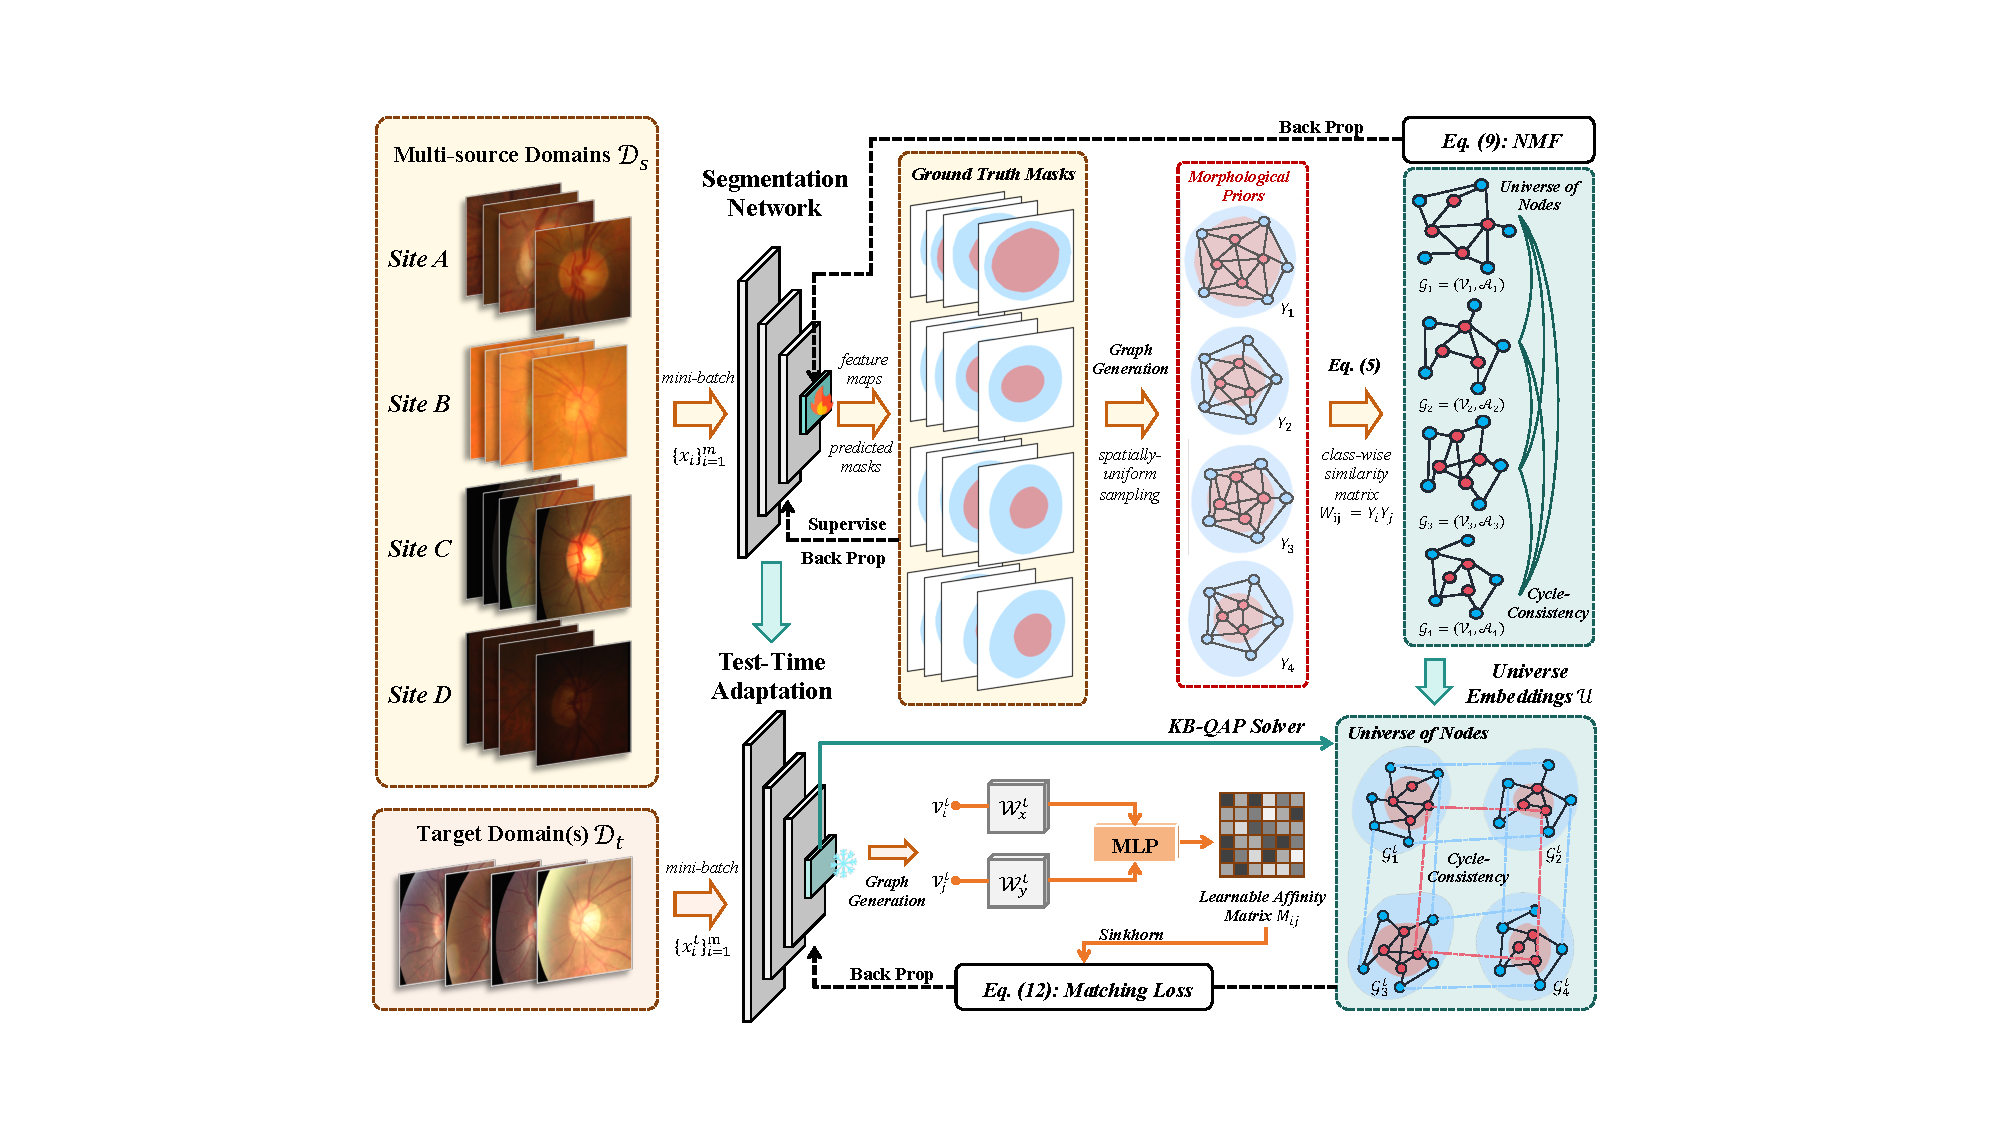
\includegraphics[width=0.98\linewidth]{Figures/pipeline_final.pdf}
    % \vspace{-10pt}
    \caption{\textbf{Overview of our TTDG framework.} During source model training, data from different domains are jointly used to train the Segmentation Network (feature extractor and segmentation head). Feature maps and ground truth masks are utilized to construct graphs $\mathcal{G}_i$ ($i=4$ in this figure legend) and corresponding labels $Y_i$ (Sec.~\ref{sec:graph_generation}), with universe embeddings learned via back-propagation, incorporating morphological priors (Sec.~\ref{sec:training}).
    At test time, multi-graph matching is performed on all target domain images in each batch. Despite style differences, these images share common morphological patterns. Universe embeddings are frozen as prior knowledge to guide the matching, and the segmentation network is fine-tuned via back-propagation for efficient adaptation (Sec.~\ref{sec:testing}).}
     \vspace{-0.5cm}
    \label{fig:pipeline}
\end{figure*}
This section provides an overview of how multi-graph matching methods can facilitate training for TTDG tasks. Given inputs consisting of images from $S$ source domains $(S \ge 1)$, denoted as $\mathcal{D}_s = \{ D_1, D_2, \cdots, D_S \}$, the objective is to enable the model to make more accurate predictions on $T$ unseen target domains $ (T\ge 1)$, denoted as $\mathcal{D}_t = \{ D_1, D_2, \cdots, D_T \}$, during the testing phase.
% First, we will introduce the preliminaries about the multi-graph matching. Subsequently, we will examine the pre-training process on $\mathcal{D}_s$ and the unsupervised multi-graph matching adaptation scheme employed during test-time for $\mathcal{D}_t$. Finally, a theoretical analysis will be provided.

Inspired by~\cite{pmlr-v235-pu24b}, we aim to effectively leverage morphological prior through graph construction. However, unlike the UDA tasks, which typically involve only two domains, our training process simultaneously handles multiple labeled domains. Pairwise matching across multiple domains can lead to the challenges discussed in Sec.~\ref{sec:intro}. To tackle this, we propose learning domain-invariant latent representations from a multi-graph matching perspective, thereby facilitating rapid adaptation to unseen domains during the TTA phase.


\subsection{Construction of Graph}
\label{sec:graph_generation}

% \noindent \textbf{Graph Generation.} 
% In contrast to conventional graph matching algorithms that rely on explicitly defined keypoints as graph nodes~\cite{gao2021deep,wang2019learning,wang2021neural},
% % our approach takes a different route. 
% accurately annotating keypoints is not only more expensive but also less practical compared to natural images in medical imaging.
Rather than using conventional graph-matching algorithms that depend on explicitly defined keypoints as graph nodes~\cite{gao2021deep,wang2019learning,wang2021neural}, accurately annotating keypoints in medical imaging is both more costly and less practical than in natural images.
Therefore, given a mini-batch $\{x_i\}_{i=1}^{m} \in \mathcal{D}_s$, as shown in Fig.~\ref{fig:pipeline}, it is first passed through a general feature extractor, such as ResNet~\cite{he2016deep}, to obtain visual features.
% for each graph $ \mathcal{G}_i$, we start by using a general feature extractor, such as ResNet~\cite{}, to obtain visual features. 
We then perform spatially-uniform sampling~\cite{li2022sigma} of pixels within the ground-truth masks at each feature level to obtain $n_i$ foreground nodes with its corresponding labels ${Y}_i\in \mathbb{Z}^{n_i}$.
After extracting these fine-grained visual features, we employ a nonlinear projection to transform the visual space into the $h$-dimensional graph space. This approach generates the feature of nodes $\{\mathcal{V}_i\in \mathbb{R}^{n_i \times h}\}_{i=1}^m$ that more effectively preserve the semantic characteristics. 
%By doing so, our method avoids the constraints of manual keypoint annotation while ensuring that the graph nodes capture meaningful visual and spatial information that is well-suited to medical imaging tasks.

For the weighted adjacency matrix encoding structural information, we use Dropedge~\cite{rongdropedge} to reduce potential bias caused by the frequent visual correspondences, preventing the model from over-relying on specific matches. The formulation is as follows:
\begin{equation}
    \mathcal{A}_i = Dropedge\{ softmax[\mathcal{V}_i \mathcal{W}_{x}\cdot(\mathcal{V}_i \mathcal{W}_{y})^{\mathsf{T}}]\odot D^{-1}\},
\end{equation}
where $\mathcal{W}_{x}$ and $\mathcal{W}_{y}$ are two learnable linear projection, $D=\frac{\mathcal{V}_i \mathcal{V}_i^{\mathsf{T}}}{||\mathcal{V}_i||_2}$ is the cosine distance matrix. Edges with larger weights indicate nodes that are closer to each other, so we use the inverse of $D$ and apply the hadamard product $\odot$ to combine node similarity with geometric proximity. The diagonal elements of $\mathcal{A}_i$ are set to zero. Based on the above steps, we obtain a corresponding graph $ \mathcal{G}_i=(\mathcal{V}_i, \mathcal{A}_i)$ for each input $x_i$. 


\subsection{Formulation of the Universe Embeddings}
\label{sec:training}
% Training Paradigm on the Source Domains
% \noindent \textbf{Universe Nodes Formulation.} 
% Different from~\cite{nurlanov2023universe}, our approach introduces geometric priors specific to medical images into the learning of universe embeddings $\mathcal{U}$. This enables the model to generate latent representations that are more attuned to the modalities of medical imaging. By incorporating these domain-specific priors, our method ensures that the learned representations better capture the stable anatomical structures and spatial layouts inherent to medical images. This design not only improves the accuracy of cross-domain tasks like segmentation and detection but also facilitates more robust knowledge transfer between different medical imaging domains, enhancing generalization to unseen domains.
In Sec.~\ref{lemma1}, it was demonstrated that by matching each node of a graph to the \textit{universe of nodes}, we can maintain cycle-consistency while avoiding the computational burden associated with cubic non-convex constraints. While a randomly initialized matrix can learn accurate universe matchings $\mathbb{U}_{n_id}$ in a supervised setting, we introduce universe embeddings $\mathcal{U} \in \mathbb{R}^{d\times h}$, which serve as learnable latent representations to enhance adaptability in unsupervised multi-domain scenarios.

$\mathcal{U}$ is initialized as $1/d + 10^{-3}z$, where $z \sim N(0, 1)$, following the setting in~\cite{wang2020graduated}. For each $\mathcal{G}_i$, we learn a unique matching between nodes in $\mathcal{V}_i$ and the corresponding in the \textit{universe of nodes}, as follows: $U_i = Sinkhorn(\mathcal{V}_i \ \mathcal{U}^{\mathsf{T}}, \tau) \in \mathbb{U}_{n_i d}$. $Sinkhorn(X, \tau)$ refers to the Sinkhorn algorithm~\cite{sinkhorn1964relationship,cuturi2013sinkhorn}, which applies a relaxed projection with entropic regularization~\cite{gold1996softmax} to normalize the matrix $X$, resulting in a doubly-stochastic matrix, and $\tau \in (0,+\infty)$ is the regularization factor. For the obtained $U_i$, the $d\times d$ matrix $U_i^{\mathsf{T}} \mathcal{A}_i U_i$ is a row and column reordering of $\mathcal{A}_i$ based on the \textit{universe of nodes}. Accordingly, the agreement between two adjacency matrices $\mathcal{A}_i$ and $\mathcal{A}_j$, reordered according to their respective universe matching assignment matrices $U_i$ and $U_j$, can be quantified using the Frobenius inner product namely $\langle U_i^{\mathsf{T}} \mathcal{A}_i U_i, U_j^{\mathsf{T}} \mathcal{A}_j U_j\rangle$. Let $\bold{U} = [U_1^{\mathsf{T}}, \cdots, U_m^{\mathsf{T}}]^{\mathsf{T}} \in \mathbb{R}^{n\times d}$, where $n = \sum_{i=1}^{m}n_i$. The block-diagonal multi-adjacency matrix is defined as $\bold{A} = diag(\mathcal{A}_1, \cdots, \mathcal{A}_m) \in \mathbb{R}^{n\times n}$. We can get the multi-matching formulation as:
\vspace{-5pt}
\begin{align}
    f(\bold{U}) := &\ \underset{U_1, \dots, U_m}{\max} \quad \sum_{i,j \in [m]} \langle U_i^{\mathsf{T}} \mathcal{A}_i U_i, U_j^{\mathsf{T}} \mathcal{A}_j U_j \rangle \nonumber \\ 
     = &\quad \underset{\bold{U} \in \mathbb{U}}{\max} \quad \text{tr}(\bold{U}^{\mathsf{T}} \bold{A} \bold{U} \bold{U}^{\mathsf{T}} \bold{A} \bold{U}) \label{eq6}.
\end{align}
% We observed that in the original multi-graph matching optimization problem~\cite{}, the matching structure in $\bold{U}$ often fails to sufficiently emphasize geometric objects with high similarity scores. To address this limitation, we introduce \textit{a label-wise similarity matrix} $\bold{W}$ to better capture and enhance these geometric relationships. This is achieved by assigning greater weight to high-similarity structure matches while suppressing lower-similarity ones. 

It was observed that in the original multi-graph matching optimization problem, graphs are typically constructed for each individual instance, with all the nodes within a graph belonging to the same category. However, in medical imaging, constructing separate graphs for each organ would not only greatly increase the computational complexity of graph matching but also result in misalignments between graphs from different categories, significantly compromising matching accuracy. To address this limitation, we introduce a \textit{class-wise similarity matrix} $\bold{W}$ to incorporate class-aware label information for each node. This ensures that the nodes are correctly aligned according to their respective categories during multi-graph matching.
Specifically, we define $W_{ij} = {Y}_i {Y}_j^{\mathsf{T}} $ and $\bold{W} = [W_{ij}]_{ij} \in \mathbb{Z}^{(\sum_{i=1}^{m}n_i)\times(\sum_{j=1}^{m}n_j)}$. The class-aware similarity matrix $\bold{\tilde{A}} = \bold{W}^{\mathsf{T}} \bold{A}\bold{W}$. Consequently, Eq. (\ref{eq6}) can be transformed into the following form
\vspace{-5pt}
\begin{equation}
    \underset{\bold{U} \in \mathbb{U}}{\max} \quad \text{tr}(\bold{U}^{\mathsf{T}} \bold{\tilde{A}} \bold{U} \bold{U}^{\mathsf{T}} \bold{\tilde{A}} \bold{U}).
\end{equation}

% The higher-order projected power iteration (HiPPI)~\cite{bernard2019hippi}, is employed to iteratively solve for $\bold{U}^*_\lim_t$
% ensuring the learning of geometric priors for medical images under cycle-consistent constraints. 
% In order to guarantee the optimal learning of universe embeddings $\mathcal{U}$, we introduce the non-negative matrix factorisation (NMF)~\cite{} $L_{con}$:
% \begin{equation}
%     L_{con} = \sum_{i,j\in [m]} ||U_i U_j^{-1} - I ||^2_F + \alpha ||\bold{U}||_F^2,
% \end{equation}
% where $I$ is the identity matrix, $||\cdot||^2_F$ represents the Frobenius norm, and $\alpha$ is a tuning parameter. The first term enforces a consistency constraint to ensure global alignment across $\mathcal{G}_1,\cdots, \mathcal{G}_m$, while the second term serves as a regularization term to maintain the numerical stability of $\bold{U}$.
% For a detailed account of the aforementioned process, please refer to Algo.~\ref{}.

The higher-order projected power iteration (HiPPI)~\cite{bernard2019hippi} is employed to iteratively solve $\bold{U}$ to obtain a stable convergence form:
\vspace{-5pt}
\begin{equation}
    U_i^\ast = U^t_i \quad s.t. \quad || U^t_i - U^{t-1}_i|| < \theta, \quad \forall i \in [m].
\end{equation}

Empirically, we set the convergence threshold $\theta=10^{-5}$. In order to guarantee the optimal learning of universe embeddings $\mathcal{U}$, we incorporate the \textit{non-negative matrix factorisation} (NMF)~\cite{lee1999learning,bernard2019synchronisation} and define the overall optimization objective as: 
\vspace{-5pt}
\begin{equation}
    L(\mathcal{U}) = \sum_{i\in [m]} || {U}^\ast_i - \mathcal{V}_i \ \mathcal{U}^{\mathsf{T}} ||^2_F + \alpha ||\mathcal{U} ||_F^2,
\end{equation}
where $||\cdot||^2_F$ represents the Frobenius norm, and $\alpha$ is a tuning parameter. Since only matrix multiplication and element-wise division are involved, the Sinkhorn operation is fully differentiable. This allows for effective updates to $\mathcal{U}$ through back-propagation, enabling the incorporation of morphological prior knowledge.

\subsection{Testing Paradigm on the Target Domains}
\label{sec:testing}
During the Test-Time Adaptation (TTA) phase, we only have access to unlabeled data from the unseen target domains $\mathcal{D}_t$. Due to distribution shifts, the performance of models trained on $\mathcal{D}_s$ can degrade significantly. To address this issue, we employ the multi-graph matching on each mini-batch $\{x_i^t\}_{i=1}^{m} \in \mathcal{D}_t$. By utilizing universe embeddings $\mathcal{U}$ learned from $\mathcal{D}_s$ as described in Sec.~\ref{sec:training}, it is guaranteed cycle-consistency, enabling the network to focus on domain-invariant features guided by morphological priors from medical images. 
In this phase, $\mathcal{U}$ is frozen to prevent error accumulation from affecting the prior information. The feature extractor and segmentation head (segmentation network in Fig.~\ref{fig:pipeline}) are optimized through gradient back-propagation, allowing the model to adapt effectively to the new domains.
% The entire process is optimized through gradient back-propagation, which enables the model to adapt effectively to the new domains. 
% given a mini-batch $\{x_i\}_{i=1}^{M} \in \mathcal{D}_t$, as shown in Fig.~\ref{}, it is first passed through the segmentation network trained on $\mathcal{D}_t$ to obtain the feature maps and predicted masks.

\noindent \textbf{Unsupervised Multi-Matching.} Following the same graph construction described in Sec.~\ref{sec:graph_generation}, we obtain the $\mathcal{G}_i^t = (\mathcal{V}_i^t, \mathcal{A}_i^t)$ for each $x_i^t$, where $\mathcal{V}_i^t \in \mathbb{R}^{n_i\times h}$ represents the $n_i$ class-aware nodes and $\mathcal{A}_i^t \in \mathbb{R}^{n_i\times n_i}$ is the adjacency matrix encoding the structural information. 
% Many DA methods rely on the model's predicted pseudo-labels 
% $\bold{Y}$ as supervision for training~\cite{}. However, using inherently incorrect predictions to supervise the training process tends to accumulate errors further. To avoid this issue, 
We first introduce a network-learned affinity matrix $M_{ij} = f_{mlp}\{\mathcal{V}_i^t \mathcal{W}_{x}^t\cdot(\mathcal{V}_j^t \mathcal{W}_{y}^t)^{\mathsf{T}}\} \in \mathbb{R}^{n_i\times n_j}$ in graph pair $\mathcal{G}_i$ and $\mathcal{G}_j$, which computes the similarity between their corresponding node features. $\mathcal{W}_{x}^t$ and $\mathcal{W}_{y}^t$ are two learnable linear projection, $f_{mlp}$ is a multi-layer perception (MLP). Subsequently, the matching between $\mathcal{G}_i$ and the universe of size $d$ is obtained through the inner-product between $\mathcal{V}_i^t$ and the pre-trained universe embeddings $\mathcal{U}$, in accordance with the same procedure $U_i = Sinkhorn(\mathcal{V}_i^t \ \mathcal{U}^{\mathsf{T}}, \tau) \in \mathbb{U}_{n_i d}$ in Sec.~\ref{sec:training}.

In~\cite{wang2020graduated,wang2023unsupervised}, the authors propose solving the multi-matching KB-QAP problem presented in Eq. (\ref{eq:mgqap}) (denoted as $J$) using a Taylor expansion. Based on the assumptions in \textit{Lemma 1} of Sec.~\ref{lemma1}, we can reformulate $J$ in Taylor series as follows:
% \begin{align}
%     J \approx & \sum_{i,j \in [m]} \lambda \ \text{tr}(U_j^0 U_i^{0T} \mathcal{A}_i U_i^0 U_j^{0T} \mathcal{A}_j) 
%     + \text{tr}(U_j^0 U_i^{0T} W_{ij}) \nonumber \\
%     & + \sum_{i \in [m]} \text{tr}\left(\frac{\partial J}{\partial U_i} \bigg|_{U_i=U_i^0} (U_i - U_i^0)\right) + \cdots
% \end{align}
\vspace{-5pt}
\begin{equation}
    J(U) \approx J(U^0) + \sum_i \frac{\partial J}{\partial U_i} \bigg|_{U=U^0} (U_i-U_i^0) + \cdots.
\end{equation}

$J$ can be approximated as $m$ linear optimization problems through the first-order Taylor expansion, which can be efficiently solved using the Sinkhorn. The gradient of $J$ with respect to $U_i$, denoted as
\vspace{-5pt}
\begin{equation}
\label{eq:v}
    V_i = \frac{\partial J}{\partial U_i} = \sum_{j\in [m]} (\lambda \mathcal{A}_i U_i U_j^{\mathsf{T}} \mathcal{A}_j U_j + M_{ij} U_j),
\end{equation}
$V_i$ ensures that $U_i$ gradually converges to a high-quality discrete solution.

Finally, the converged $\{U_i\}$ fine-tune the segmentation network with the matching loss $L_{mat}$: 
\vspace{-5pt}
\begin{align}
    L_{mat} = & \sum_{i,j \in [m]} \left[ -\hat{M}_{ij}^\gamma (1 - U_i U_j^{\mathsf{T}}) \log(U_i U_j^{\mathsf{T}}) \right] \nonumber \\
     - & \sum_{i,j \in [m]} \left[ (1 - \hat{M}_{ij})^\gamma U_i U_j^{\mathsf{T}} \log(1 - U_i U_j^{\mathsf{T}}) \right],
\end{align}
where $\hat{M}_{ij} = sinkhorn(M_{ij}, \tau)$, and $\gamma$ is an amplification factor. See algorithm in appendix for full details.